\documentclass[1p]{elsarticle_modified}
%\bibliographystyle{elsarticle-num}

%\usepackage[colorlinks]{hyperref}
%\usepackage{abbrmath_seonhwa} %\Abb, \Ascr, \Acal ,\Abf, \Afrak
\usepackage{amsfonts}
\usepackage{amssymb}
\usepackage{amsmath}
\usepackage{amsthm}
\usepackage{scalefnt}
\usepackage{amsbsy}
\usepackage{kotex}
\usepackage{caption}
\usepackage{subfig}
\usepackage{color}
\usepackage{graphicx}
\usepackage{xcolor} %% white, black, red, green, blue, cyan, magenta, yellow
\usepackage{float}
\usepackage{setspace}
\usepackage{hyperref}

\usepackage{tikz}
\usetikzlibrary{arrows}

\usepackage{multirow}
\usepackage{array} % fixed length table
\usepackage{hhline}

%%%%%%%%%%%%%%%%%%%%%
\makeatletter
\renewcommand*\env@matrix[1][\arraystretch]{%
	\edef\arraystretch{#1}%
	\hskip -\arraycolsep
	\let\@ifnextchar\new@ifnextchar
	\array{*\c@MaxMatrixCols c}}
\makeatother %https://tex.stackexchange.com/questions/14071/how-can-i-increase-the-line-spacing-in-a-matrix
%%%%%%%%%%%%%%%

\usepackage[normalem]{ulem}

\newcommand{\msout}[1]{\ifmmode\text{\sout{\ensuremath{#1}}}\else\sout{#1}\fi}
%SOURCE: \msout is \stkout macro in https://tex.stackexchange.com/questions/20609/strikeout-in-math-mode

\newcommand{\cancel}[1]{
	\ifmmode
	{\color{red}\msout{#1}}
	\else
	{\color{red}\sout{#1}}
	\fi
}

\newcommand{\add}[1]{
	{\color{blue}\uwave{#1}}
}

\newcommand{\replace}[2]{
	\ifmmode
	{\color{red}\msout{#1}}{\color{blue}\uwave{#2}}
	\else
	{\color{red}\sout{#1}}{\color{blue}\uwave{#2}}
	\fi
}

\newcommand{\Sol}{\mathcal{S}} %segment
\newcommand{\D}{D} %diagram
\newcommand{\A}{\mathcal{A}} %arc


%%%%%%%%%%%%%%%%%%%%%%%%%%%%%5 test

\def\sl{\operatorname{\textup{SL}}(2,\Cbb)}
\def\psl{\operatorname{\textup{PSL}}(2,\Cbb)}
\def\quan{\mkern 1mu \triangleright \mkern 1mu}

\theoremstyle{definition}
\newtheorem{thm}{Theorem}[section]
\newtheorem{prop}[thm]{Proposition}
\newtheorem{lem}[thm]{Lemma}
\newtheorem{ques}[thm]{Question}
\newtheorem{cor}[thm]{Corollary}
\newtheorem{defn}[thm]{Definition}
\newtheorem{exam}[thm]{Example}
\newtheorem{rmk}[thm]{Remark}
\newtheorem{alg}[thm]{Algorithm}

\newcommand{\I}{\sqrt{-1}}
\begin{document}

%\begin{frontmatter}
%
%\title{Boundary parabolic representations of knots up to 8 crossings}
%
%%% Group authors per affiliation:
%\author{Yunhi Cho} 
%\address{Department of Mathematics, University of Seoul, Seoul, Korea}
%\ead{yhcho@uos.ac.kr}
%
%
%\author{Seonhwa Kim} %\fnref{s_kim}}
%\address{Center for Geometry and Physics, Institute for Basic Science, Pohang, 37673, Korea}
%\ead{ryeona17@ibs.re.kr}
%
%\author{Hyuk Kim}
%\address{Department of Mathematical Sciences, Seoul National University, Seoul 08826, Korea}
%\ead{hyukkim@snu.ac.kr}
%
%\author{Seokbeom Yoon}
%\address{Department of Mathematical Sciences, Seoul National University, Seoul, 08826,  Korea}
%\ead{sbyoon15@snu.ac.kr}
%
%\begin{abstract}
%We find all boundary parabolic representation of knots up to 8 crossings.
%
%\end{abstract}
%\begin{keyword}
%    \MSC[2010] 57M25 
%\end{keyword}
%
%\end{frontmatter}

%\linenumbers
%\tableofcontents
%
\newcommand\colored[1]{\textcolor{white}{\rule[-0.35ex]{0.8em}{1.4ex}}\kern-0.8em\color{red} #1}%
%\newcommand\colored[1]{\textcolor{white}{ #1}\kern-2.17ex	\textcolor{white}{ #1}\kern-1.81ex	\textcolor{white}{ #1}\kern-2.15ex\color{red}#1	}

{\Large $\underline{12n_{0807}~(K12n_{0807})}$}

\setlength{\tabcolsep}{10pt}
\renewcommand{\arraystretch}{1.6}
\vspace{1cm}\begin{tabular}{m{100pt}>{\centering\arraybackslash}m{274pt}}
\multirow{5}{120pt}{
	\centering
	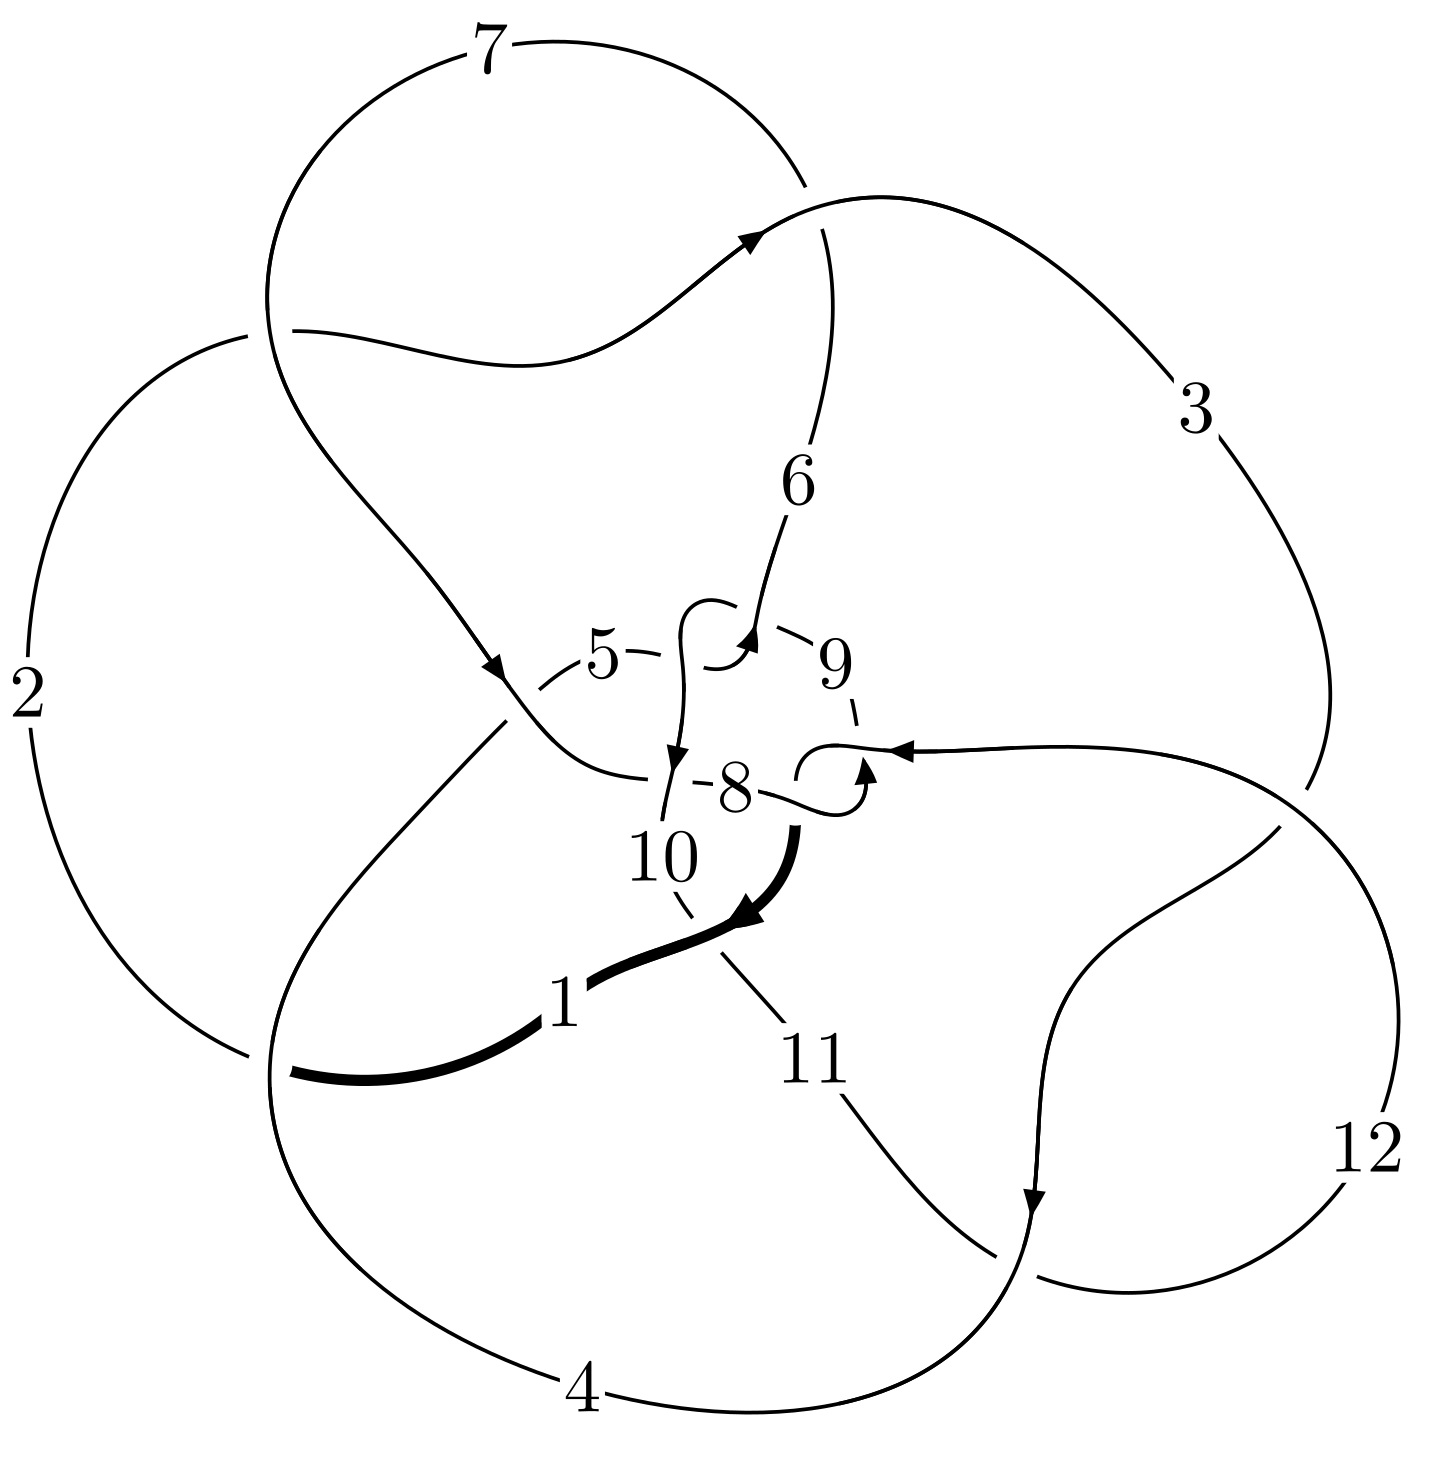
\includegraphics[width=112pt]{../../../GIT/diagram.site/Diagrams/png/2896_12n_0807.png}\\
\ \ \ A knot diagram\footnotemark}&
\allowdisplaybreaks
\textbf{Linearized knot diagam} \\
\cline{2-2}
 &
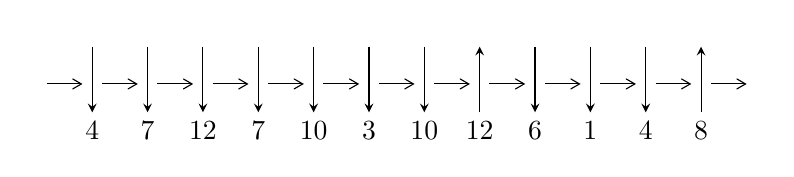
\begin{tikzpicture}[x=20pt, y=17pt]
	% nodes
	\node (C0) at (0, 0) {};
	\node (C1) at (1, 0) {};
	\node (C1U) at (1, +1) {};
	\node (C1D) at (1, -1) {4};

	\node (C2) at (2, 0) {};
	\node (C2U) at (2, +1) {};
	\node (C2D) at (2, -1) {7};

	\node (C3) at (3, 0) {};
	\node (C3U) at (3, +1) {};
	\node (C3D) at (3, -1) {12};

	\node (C4) at (4, 0) {};
	\node (C4U) at (4, +1) {};
	\node (C4D) at (4, -1) {7};

	\node (C5) at (5, 0) {};
	\node (C5U) at (5, +1) {};
	\node (C5D) at (5, -1) {10};

	\node (C6) at (6, 0) {};
	\node (C6U) at (6, +1) {};
	\node (C6D) at (6, -1) {3};

	\node (C7) at (7, 0) {};
	\node (C7U) at (7, +1) {};
	\node (C7D) at (7, -1) {10};

	\node (C8) at (8, 0) {};
	\node (C8U) at (8, +1) {};
	\node (C8D) at (8, -1) {12};

	\node (C9) at (9, 0) {};
	\node (C9U) at (9, +1) {};
	\node (C9D) at (9, -1) {6};

	\node (C10) at (10, 0) {};
	\node (C10U) at (10, +1) {};
	\node (C10D) at (10, -1) {1};

	\node (C11) at (11, 0) {};
	\node (C11U) at (11, +1) {};
	\node (C11D) at (11, -1) {4};

	\node (C12) at (12, 0) {};
	\node (C12U) at (12, +1) {};
	\node (C12D) at (12, -1) {8};
	\node (C13) at (13, 0) {};

	% arrows
	\draw[->,>={angle 60}]
	(C0) edge (C1) (C1) edge (C2) (C2) edge (C3) (C3) edge (C4) (C4) edge (C5) (C5) edge (C6) (C6) edge (C7) (C7) edge (C8) (C8) edge (C9) (C9) edge (C10) (C10) edge (C11) (C11) edge (C12) (C12) edge (C13) ;	\draw[->,>=stealth]
	(C1U) edge (C1D) (C2U) edge (C2D) (C3U) edge (C3D) (C4U) edge (C4D) (C5U) edge (C5D) (C6U) edge (C6D) (C7U) edge (C7D) (C8D) edge (C8U) (C9U) edge (C9D) (C10U) edge (C10D) (C11U) edge (C11D) (C12D) edge (C12U) ;
	\end{tikzpicture} \\
\hhline{~~} \\& 
\textbf{Solving Sequence} \\ \cline{2-2} 
 &
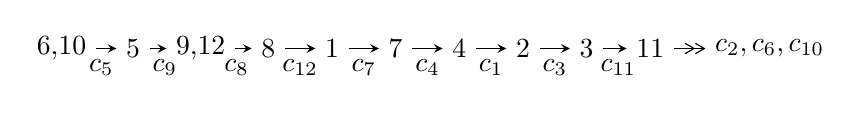
\begin{tikzpicture}[x=23pt, y=7pt]
	% node
	\node (A0) at (-1/8, 0) {6,10};
	\node (A1) at (1, 0) {5};
	\node (A2) at (33/16, 0) {9,12};
	\node (A3) at (25/8, 0) {8};
	\node (A4) at (33/8, 0) {1};
	\node (A5) at (41/8, 0) {7};
	\node (A6) at (49/8, 0) {4};
	\node (A7) at (57/8, 0) {2};
	\node (A8) at (65/8, 0) {3};
	\node (A9) at (73/8, 0) {11};
	\node (C1) at (1/2, -1) {$c_{5}$};
	\node (C2) at (3/2, -1) {$c_{9}$};
	\node (C3) at (21/8, -1) {$c_{8}$};
	\node (C4) at (29/8, -1) {$c_{12}$};
	\node (C5) at (37/8, -1) {$c_{7}$};
	\node (C6) at (45/8, -1) {$c_{4}$};
	\node (C7) at (53/8, -1) {$c_{1}$};
	\node (C8) at (61/8, -1) {$c_{3}$};
	\node (C9) at (69/8, -1) {$c_{11}$};
	\node (A10) at (11, 0) {$c_{2},c_{6},c_{10}$};

	% edge
	\draw[->,>=stealth]	
	(A0) edge (A1) (A1) edge (A2) (A2) edge (A3) (A3) edge (A4) (A4) edge (A5) (A5) edge (A6) (A6) edge (A7) (A7) edge (A8) (A8) edge (A9) ;
	\draw[->>,>={angle 60}]	
	(A9) edge (A10);
\end{tikzpicture} \\ 

\end{tabular} \\

\footnotetext{
The image of knot diagram is generated by the software ``\textbf{Draw programme}" developed by Andrew Bartholomew(\url{http://www.layer8.co.uk/maths/draw/index.htm\#Running-draw}), where we modified some parts for our purpose(\url{https://github.com/CATsTAILs/LinksPainter}).
}\phantom \\ \newline 
\centering \textbf{Ideals for irreducible components\footnotemark of $X_{\text{par}}$} 
 
\begin{align*}
I^u_{1}&=\langle 
12477565171 u^{19}-2707721730 u^{18}+\cdots+64702086776 b+27595919604,\\
\phantom{I^u_{1}}&\phantom{= \langle  }78169757719 u^{19}-30849689152 u^{18}+\cdots+129404173552 a+57487393140,\\
\phantom{I^u_{1}}&\phantom{= \langle  }u^{20}- u^{19}+\cdots-24 u+4\rangle \\
I^u_{2}&=\langle 
-2.57900\times10^{40} u^{27}+3.53622\times10^{40} u^{26}+\cdots+9.02119\times10^{41} b-2.68374\times10^{42},\\
\phantom{I^u_{2}}&\phantom{= \langle  }-1.76496\times10^{42} u^{27}+2.49630\times10^{42} u^{26}+\cdots+8.57013\times10^{43} a-4.54812\times10^{44},\\
\phantom{I^u_{2}}&\phantom{= \langle  }u^{28}- u^{27}+\cdots+95 u+25\rangle \\
I^u_{3}&=\langle 
- u^5-2 u^4-3 u^3+2 b+u+1,\;u^3+u^2+a+2 u-1,\;u^6+u^5+3 u^4- u^3+u^2-2 u+1\rangle \\
I^u_{4}&=\langle 
6613602 u^{13}+3587729 u^{12}+\cdots+4472398 b+51425184,\\
\phantom{I^u_{4}}&\phantom{= \langle  }7928755 u^{13}+5002338 u^{12}+\cdots+8944796 a+66385836,\\
\phantom{I^u_{4}}&\phantom{= \langle  }u^{14}+u^{12}+3 u^{11}-7 u^{10}- u^9+5 u^8-6 u^7+u^6+u^5+u^4+12 u^3-22 u^2+16 u-4\rangle \\
\\
\end{align*}
\raggedright * 4 irreducible components of $\dim_{\mathbb{C}}=0$, with total 68 representations.\\
\footnotetext{All coefficients of polynomials are rational numbers. But the coefficients are sometimes approximated in decimal forms when there is not enough margin.}
\newpage
\renewcommand{\arraystretch}{1}
\centering \section*{I. $I^u_{1}= \langle 1.25\times10^{10} u^{19}-2.71\times10^{9} u^{18}+\cdots+6.47\times10^{10} b+2.76\times10^{10},\;7.82\times10^{10} u^{19}-3.08\times10^{10} u^{18}+\cdots+1.29\times10^{11} a+5.75\times10^{10},\;u^{20}- u^{19}+\cdots-24 u+4 \rangle$}
\flushleft \textbf{(i) Arc colorings}\\
\begin{tabular}{m{7pt} m{180pt} m{7pt} m{180pt} }
\flushright $a_{6}=$&$\begin{pmatrix}1\\0\end{pmatrix}$ \\
\flushright $a_{10}=$&$\begin{pmatrix}0\\u\end{pmatrix}$ \\
\flushright $a_{5}=$&$\begin{pmatrix}1\\- u^2\end{pmatrix}$ \\
\flushright $a_{9}=$&$\begin{pmatrix}u\\u\end{pmatrix}$ \\
\flushright $a_{12}=$&$\begin{pmatrix}-0.604074 u^{19}+0.238398 u^{18}+\cdots-4.76779 u-0.444247\\-0.192846 u^{19}+0.0418491 u^{18}+\cdots+1.83993 u-0.426507\end{pmatrix}$ \\
\flushright $a_{8}=$&$\begin{pmatrix}0.516386 u^{19}-0.359863 u^{18}+\cdots+5.34580 u+0.660241\\0.0583155 u^{19}-0.180402 u^{18}+\cdots+4.96135 u-0.712465\end{pmatrix}$ \\
\flushright $a_{1}=$&$\begin{pmatrix}-0.516386 u^{19}+0.359863 u^{18}+\cdots-5.34580 u-0.660241\\-0.125103 u^{19}+0.150575 u^{18}+\cdots-3.16402 u+0.759990\end{pmatrix}$ \\
\flushright $a_{7}=$&$\begin{pmatrix}0.516386 u^{19}-0.359863 u^{18}+\cdots+5.34580 u+0.660241\\0.179296 u^{19}-0.251320 u^{18}+\cdots+3.27034 u-0.0863736\end{pmatrix}$ \\
\flushright $a_{4}=$&$\begin{pmatrix}-0.298481 u^{19}+0.162206 u^{18}+\cdots-4.44207 u+1.60482\\-0.190429 u^{19}+0.224600 u^{18}+\cdots-4.91842 u+0.679023\end{pmatrix}$ \\
\flushright $a_{2}=$&$\begin{pmatrix}-0.0233919 u^{19}+0.141504 u^{18}+\cdots-0.574180 u-1.17094\\0.0994137 u^{19}-0.225778 u^{18}+\cdots+6.99444 u-0.952482\end{pmatrix}$ \\
\flushright $a_{3}=$&$\begin{pmatrix}0.0671954 u^{19}-0.268402 u^{18}+\cdots+10.5000 u-0.811473\\-0.0394315 u^{19}+0.0310711 u^{18}+\cdots+0.136398 u-0.0923623\end{pmatrix}$ \\
\flushright $a_{11}=$&$\begin{pmatrix}-0.740350 u^{19}+0.510891 u^{18}+\cdots-10.3265 u+0.749678\\-0.158675 u^{19}+0.234881 u^{18}+\cdots-2.05133 u+0.335208\end{pmatrix}$\\&\end{tabular}
\flushleft \textbf{(ii) Obstruction class $= -1$}\\~\\
\flushleft \textbf{(iii) Cusp Shapes $= \frac{28600507011}{16175521694} u^{19}-\frac{9150517238}{8087760847} u^{18}+\cdots+\frac{468797321056}{8087760847} u-\frac{126502436106}{8087760847}$}\\~\\
\newpage\renewcommand{\arraystretch}{1}
\flushleft \textbf{(iv) u-Polynomials at the component}\newline \\
\begin{tabular}{m{50pt}|m{274pt}}
Crossings & \hspace{64pt}u-Polynomials at each crossing \\
\hline $$\begin{aligned}c_{1},c_{4}\end{aligned}$$&$\begin{aligned}
&u^{20}-2 u^{19}+\cdots-14 u+1
\end{aligned}$\\
\hline $$\begin{aligned}c_{2},c_{6}\end{aligned}$$&$\begin{aligned}
&u^{20}+5 u^{19}+\cdots+28 u+10
\end{aligned}$\\
\hline $$\begin{aligned}c_{3},c_{5},c_{9}\\c_{11}\end{aligned}$$&$\begin{aligned}
&u^{20}+u^{19}+\cdots+24 u+4
\end{aligned}$\\
\hline $$\begin{aligned}c_{7},c_{10}\end{aligned}$$&$\begin{aligned}
&u^{20}- u^{19}+\cdots+9 u+1
\end{aligned}$\\
\hline $$\begin{aligned}c_{8},c_{12}\end{aligned}$$&$\begin{aligned}
&u^{20}-8 u^{19}+\cdots+26 u-14
\end{aligned}$\\
\hline
\end{tabular}\\~\\
\newpage\renewcommand{\arraystretch}{1}
\flushleft \textbf{(v) Riley Polynomials at the component}\newline \\
\begin{tabular}{m{50pt}|m{274pt}}
Crossings & \hspace{64pt}Riley Polynomials at each crossing \\
\hline $$\begin{aligned}c_{1},c_{4}\end{aligned}$$&$\begin{aligned}
&y^{20}-30 y^{19}+\cdots+10 y+1
\end{aligned}$\\
\hline $$\begin{aligned}c_{2},c_{6}\end{aligned}$$&$\begin{aligned}
&y^{20}+7 y^{19}+\cdots-744 y+100
\end{aligned}$\\
\hline $$\begin{aligned}c_{3},c_{5},c_{9}\\c_{11}\end{aligned}$$&$\begin{aligned}
&y^{20}+19 y^{19}+\cdots+80 y+16
\end{aligned}$\\
\hline $$\begin{aligned}c_{7},c_{10}\end{aligned}$$&$\begin{aligned}
&y^{20}-17 y^{19}+\cdots-121 y+1
\end{aligned}$\\
\hline $$\begin{aligned}c_{8},c_{12}\end{aligned}$$&$\begin{aligned}
&y^{20}-4 y^{19}+\cdots-1516 y+196
\end{aligned}$\\
\hline
\end{tabular}\\~\\
\newpage\flushleft \textbf{(vi) Complex Volumes and Cusp Shapes}
$$\begin{array}{c|c|c}  
\text{Solutions to }I^u_{1}& \I (\text{vol} + \sqrt{-1}CS) & \text{Cusp shape}\\
 \hline 
\begin{aligned}
u &= \phantom{-}1.12905\phantom{ +0.000000I} \\
a &= -0.359607\phantom{ +0.000000I} \\
b &= -1.01716\phantom{ +0.000000I}\end{aligned}
 & -8.01665\phantom{ +0.000000I} & -11.3930\phantom{ +0.000000I} \\ \hline\begin{aligned}
u &= -0.606091 + 1.044440 I \\
a &= -0.154877 + 0.090999 I \\
b &= \phantom{-}0.246614 + 0.948938 I\end{aligned}
 & \phantom{-}4.82527 - 0.08424 I & -5.01924 - 0.20177 I \\ \hline\begin{aligned}
u &= -0.606091 - 1.044440 I \\
a &= -0.154877 - 0.090999 I \\
b &= \phantom{-}0.246614 - 0.948938 I\end{aligned}
 & \phantom{-}4.82527 + 0.08424 I & -5.01924 + 0.20177 I \\ \hline\begin{aligned}
u &= \phantom{-}0.330639 + 0.692945 I \\
a &= \phantom{-}1.36926 + 1.04069 I \\
b &= -0.252443 + 1.228440 I\end{aligned}
 & -6.44427 + 0.93056 I & -10.49794 - 0.14511 I \\ \hline\begin{aligned}
u &= \phantom{-}0.330639 - 0.692945 I \\
a &= \phantom{-}1.36926 - 1.04069 I \\
b &= -0.252443 - 1.228440 I\end{aligned}
 & -6.44427 - 0.93056 I & -10.49794 + 0.14511 I \\ \hline\begin{aligned}
u &= \phantom{-}0.040542 + 0.738588 I \\
a &= \phantom{-}2.28316 - 0.41519 I \\
b &= \phantom{-}0.861536 + 0.029448 I\end{aligned}
 & \phantom{-}1.19115 + 4.34933 I & -8.67394 + 0.08725 I \\ \hline\begin{aligned}
u &= \phantom{-}0.040542 - 0.738588 I \\
a &= \phantom{-}2.28316 + 0.41519 I \\
b &= \phantom{-}0.861536 - 0.029448 I\end{aligned}
 & \phantom{-}1.19115 - 4.34933 I & -8.67394 - 0.08725 I \\ \hline\begin{aligned}
u &= -0.461546 + 1.231960 I \\
a &= -0.561795 + 0.808913 I \\
b &= -0.85919 + 1.83207 I\end{aligned}
 & -4.99906 + 5.81831 I & -7.50691 - 4.95248 I \\ \hline\begin{aligned}
u &= -0.461546 - 1.231960 I \\
a &= -0.561795 - 0.808913 I \\
b &= -0.85919 - 1.83207 I\end{aligned}
 & -4.99906 - 5.81831 I & -7.50691 + 4.95248 I \\ \hline\begin{aligned}
u &= \phantom{-}0.332357 + 1.332800 I \\
a &= -0.037401 - 1.225500 I \\
b &= -0.25149 - 1.62627 I\end{aligned}
 & \phantom{-}4.23168 - 3.75806 I & -8.78905 + 3.32796 I\\
 \hline 
 \end{array}$$\newpage$$\begin{array}{c|c|c}  
\text{Solutions to }I^u_{1}& \I (\text{vol} + \sqrt{-1}CS) & \text{Cusp shape}\\
 \hline 
\begin{aligned}
u &= \phantom{-}0.332357 - 1.332800 I \\
a &= -0.037401 + 1.225500 I \\
b &= -0.25149 + 1.62627 I\end{aligned}
 & \phantom{-}4.23168 + 3.75806 I & -8.78905 - 3.32796 I \\ \hline\begin{aligned}
u &= \phantom{-}0.267001 + 0.387206 I \\
a &= -1.12051 - 1.01732 I \\
b &= -0.112063 + 0.500261 I\end{aligned}
 & -0.434096 - 1.337960 I & -3.82072 + 5.86960 I \\ \hline\begin{aligned}
u &= \phantom{-}0.267001 - 0.387206 I \\
a &= -1.12051 + 1.01732 I \\
b &= -0.112063 - 0.500261 I\end{aligned}
 & -0.434096 + 1.337960 I & -3.82072 - 5.86960 I \\ \hline\begin{aligned}
u &= \phantom{-}0.379438\phantom{ +0.000000I} \\
a &= -0.343267\phantom{ +0.000000I} \\
b &= \phantom{-}0.662281\phantom{ +0.000000I}\end{aligned}
 & -0.997451\phantom{ +0.000000I} & -8.03610\phantom{ +0.000000I} \\ \hline\begin{aligned}
u &= -0.53782 + 1.58865 I \\
a &= \phantom{-}0.217202 - 0.766665 I \\
b &= -0.04599 - 1.77133 I\end{aligned}
 & \phantom{-}8.99311 + 1.97630 I & -1.32435 - 3.05879 I \\ \hline\begin{aligned}
u &= -0.53782 - 1.58865 I \\
a &= \phantom{-}0.217202 + 0.766665 I \\
b &= -0.04599 + 1.77133 I\end{aligned}
 & \phantom{-}8.99311 - 1.97630 I & -1.32435 + 3.05879 I \\ \hline\begin{aligned}
u &= -0.65030 + 1.59655 I \\
a &= -1.028920 + 0.531678 I \\
b &= \phantom{-}0.066168 + 0.771188 I\end{aligned}
 & -2.70292 + 4.75701 I & -8.90322 - 3.07361 I \\ \hline\begin{aligned}
u &= -0.65030 - 1.59655 I \\
a &= -1.028920 - 0.531678 I \\
b &= \phantom{-}0.066168 - 0.771188 I\end{aligned}
 & -2.70292 - 4.75701 I & -8.90322 + 3.07361 I \\ \hline\begin{aligned}
u &= \phantom{-}1.03097 + 1.49136 I \\
a &= \phantom{-}0.385322 + 1.112120 I \\
b &= \phantom{-}0.52429 + 2.07473 I\end{aligned}
 & -1.7987 - 14.4623 I & -8.25030 + 6.83242 I \\ \hline\begin{aligned}
u &= \phantom{-}1.03097 - 1.49136 I \\
a &= \phantom{-}0.385322 - 1.112120 I \\
b &= \phantom{-}0.52429 - 2.07473 I\end{aligned}
 & -1.7987 + 14.4623 I & -8.25030 - 6.83242 I\\
 \hline 
 \end{array}$$\newpage\newpage\renewcommand{\arraystretch}{1}
\centering \section*{II. $I^u_{2}= \langle -2.58\times10^{40} u^{27}+3.54\times10^{40} u^{26}+\cdots+9.02\times10^{41} b-2.68\times10^{42},\;-1.76\times10^{42} u^{27}+2.50\times10^{42} u^{26}+\cdots+8.57\times10^{43} a-4.55\times10^{44},\;u^{28}- u^{27}+\cdots+95 u+25 \rangle$}
\flushleft \textbf{(i) Arc colorings}\\
\begin{tabular}{m{7pt} m{180pt} m{7pt} m{180pt} }
\flushright $a_{6}=$&$\begin{pmatrix}1\\0\end{pmatrix}$ \\
\flushright $a_{10}=$&$\begin{pmatrix}0\\u\end{pmatrix}$ \\
\flushright $a_{5}=$&$\begin{pmatrix}1\\- u^2\end{pmatrix}$ \\
\flushright $a_{9}=$&$\begin{pmatrix}u\\u\end{pmatrix}$ \\
\flushright $a_{12}=$&$\begin{pmatrix}0.0205943 u^{27}-0.0291279 u^{26}+\cdots-2.74979 u+5.30694\\0.0285882 u^{27}-0.0391990 u^{26}+\cdots-3.07837 u+2.97493\end{pmatrix}$ \\
\flushright $a_{8}=$&$\begin{pmatrix}0.0295456 u^{27}-0.0540163 u^{26}+\cdots-6.36659 u+1.04698\\0.0322136 u^{27}-0.0409569 u^{26}+\cdots+0.376791 u+1.67777\end{pmatrix}$ \\
\flushright $a_{1}=$&$\begin{pmatrix}0.0771412 u^{27}-0.0790894 u^{26}+\cdots+3.05691 u+7.47630\\0.0384494 u^{27}-0.0482680 u^{26}+\cdots-0.878749 u+4.68521\end{pmatrix}$ \\
\flushright $a_{7}=$&$\begin{pmatrix}0.0295456 u^{27}-0.0540163 u^{26}+\cdots-6.36659 u+1.04698\\0.0347077 u^{27}-0.0471353 u^{26}+\cdots-1.20929 u+1.06600\end{pmatrix}$ \\
\flushright $a_{4}=$&$\begin{pmatrix}-0.0575867 u^{27}+0.0693145 u^{26}+\cdots-2.27382 u-8.21914\\-0.0238237 u^{27}+0.0350049 u^{26}+\cdots+2.95822 u-4.74941\end{pmatrix}$ \\
\flushright $a_{2}=$&$\begin{pmatrix}-0.0752950 u^{27}+0.0687026 u^{26}+\cdots-5.09400 u-7.24933\\-0.0319712 u^{27}+0.0360560 u^{26}+\cdots-0.410280 u-4.02144\end{pmatrix}$ \\
\flushright $a_{3}=$&$\begin{pmatrix}0.0886392 u^{27}-0.0807706 u^{26}+\cdots+10.1105 u+2.87510\\0.0241381 u^{27}-0.0163375 u^{26}+\cdots+4.61411 u+2.08392\end{pmatrix}$ \\
\flushright $a_{11}=$&$\begin{pmatrix}0.186332 u^{27}-0.250049 u^{26}+\cdots-2.97174 u+16.2242\\0.125465 u^{27}-0.136882 u^{26}+\cdots+3.15967 u+12.8085\end{pmatrix}$\\&\end{tabular}
\flushleft \textbf{(ii) Obstruction class $= -1$}\\~\\
\flushleft \textbf{(iii) Cusp Shapes $= 0.153961 u^{27}-0.244058 u^{26}+\cdots-14.1573 u+5.74251$}\\~\\
\newpage\renewcommand{\arraystretch}{1}
\flushleft \textbf{(iv) u-Polynomials at the component}\newline \\
\begin{tabular}{m{50pt}|m{274pt}}
Crossings & \hspace{64pt}u-Polynomials at each crossing \\
\hline $$\begin{aligned}c_{1},c_{4}\end{aligned}$$&$\begin{aligned}
&u^{28}-2 u^{27}+\cdots+5356 u-619
\end{aligned}$\\
\hline $$\begin{aligned}c_{2},c_{6}\end{aligned}$$&$\begin{aligned}
&(u^{14}- u^{13}+\cdots+3 u-5)^{2}
\end{aligned}$\\
\hline $$\begin{aligned}c_{3},c_{5},c_{9}\\c_{11}\end{aligned}$$&$\begin{aligned}
&u^{28}+u^{27}+\cdots-95 u+25
\end{aligned}$\\
\hline $$\begin{aligned}c_{7},c_{10}\end{aligned}$$&$\begin{aligned}
&u^{28}+2 u^{27}+\cdots+170 u-53
\end{aligned}$\\
\hline $$\begin{aligned}c_{8},c_{12}\end{aligned}$$&$\begin{aligned}
&(u^{14}+3 u^{13}+\cdots+u+1)^{2}
\end{aligned}$\\
\hline
\end{tabular}\\~\\
\newpage\renewcommand{\arraystretch}{1}
\flushleft \textbf{(v) Riley Polynomials at the component}\newline \\
\begin{tabular}{m{50pt}|m{274pt}}
Crossings & \hspace{64pt}Riley Polynomials at each crossing \\
\hline $$\begin{aligned}c_{1},c_{4}\end{aligned}$$&$\begin{aligned}
&y^{28}-32 y^{27}+\cdots-2525320 y+383161
\end{aligned}$\\
\hline $$\begin{aligned}c_{2},c_{6}\end{aligned}$$&$\begin{aligned}
&(y^{14}+9 y^{13}+\cdots+271 y+25)^{2}
\end{aligned}$\\
\hline $$\begin{aligned}c_{3},c_{5},c_{9}\\c_{11}\end{aligned}$$&$\begin{aligned}
&y^{28}+y^{27}+\cdots-2075 y+625
\end{aligned}$\\
\hline $$\begin{aligned}c_{7},c_{10}\end{aligned}$$&$\begin{aligned}
&y^{28}-30 y^{27}+\cdots-14166 y+2809
\end{aligned}$\\
\hline $$\begin{aligned}c_{8},c_{12}\end{aligned}$$&$\begin{aligned}
&(y^{14}-3 y^{13}+\cdots-9 y+1)^{2}
\end{aligned}$\\
\hline
\end{tabular}\\~\\
\newpage\flushleft \textbf{(vi) Complex Volumes and Cusp Shapes}
$$\begin{array}{c|c|c}  
\text{Solutions to }I^u_{2}& \I (\text{vol} + \sqrt{-1}CS) & \text{Cusp shape}\\
 \hline 
\begin{aligned}
u &= -0.382569 + 0.961679 I \\
a &= \phantom{-}0.84193 + 1.31313 I \\
b &= \phantom{-}0.74021 + 1.62534 I\end{aligned}
 & -1.05651 + 1.71922 I & -3.54630 + 3.88789 I \\ \hline\begin{aligned}
u &= -0.382569 - 0.961679 I \\
a &= \phantom{-}0.84193 - 1.31313 I \\
b &= \phantom{-}0.74021 - 1.62534 I\end{aligned}
 & -1.05651 - 1.71922 I & -3.54630 - 3.88789 I \\ \hline\begin{aligned}
u &= -0.659980 + 0.684862 I \\
a &= -0.614643 + 0.241881 I \\
b &= \phantom{-}0.22392 + 1.79952 I\end{aligned}
 & \phantom{-}5.74683 + 3.41396 I & -10.73005 - 1.32661 I \\ \hline\begin{aligned}
u &= -0.659980 - 0.684862 I \\
a &= -0.614643 - 0.241881 I \\
b &= \phantom{-}0.22392 - 1.79952 I\end{aligned}
 & \phantom{-}5.74683 - 3.41396 I & -10.73005 + 1.32661 I \\ \hline\begin{aligned}
u &= -0.228826 + 0.744696 I \\
a &= \phantom{-}1.72758 - 0.31252 I \\
b &= -0.160568 - 0.530138 I\end{aligned}
 & -7.37370 - 3.17606 I & -3.96370 + 3.07132 I \\ \hline\begin{aligned}
u &= -0.228826 - 0.744696 I \\
a &= \phantom{-}1.72758 + 0.31252 I \\
b &= -0.160568 + 0.530138 I\end{aligned}
 & -7.37370 + 3.17606 I & -3.96370 - 3.07132 I \\ \hline\begin{aligned}
u &= \phantom{-}0.548168 + 1.129440 I \\
a &= -0.528269 - 0.526549 I \\
b &= -0.62027 - 1.83839 I\end{aligned}
 & -4.37474 - 4.68298 I & -8.16766 + 3.94230 I \\ \hline\begin{aligned}
u &= \phantom{-}0.548168 - 1.129440 I \\
a &= -0.528269 + 0.526549 I \\
b &= -0.62027 + 1.83839 I\end{aligned}
 & -4.37474 + 4.68298 I & -8.16766 - 3.94230 I \\ \hline\begin{aligned}
u &= \phantom{-}0.443597 + 1.210440 I \\
a &= -0.78830 - 1.27422 I \\
b &= -0.95981 - 2.01969 I\end{aligned}
 & \phantom{-}3.68681 - 6.62681 I & -5.84998 + 6.47809 I \\ \hline\begin{aligned}
u &= \phantom{-}0.443597 - 1.210440 I \\
a &= -0.78830 + 1.27422 I \\
b &= -0.95981 + 2.01969 I\end{aligned}
 & \phantom{-}3.68681 + 6.62681 I & -5.84998 - 6.47809 I\\
 \hline 
 \end{array}$$\newpage$$\begin{array}{c|c|c}  
\text{Solutions to }I^u_{2}& \I (\text{vol} + \sqrt{-1}CS) & \text{Cusp shape}\\
 \hline 
\begin{aligned}
u &= \phantom{-}1.295300 + 0.052096 I \\
a &= \phantom{-}0.615026 - 0.559035 I \\
b &= \phantom{-}0.420326 - 0.383474 I\end{aligned}
 & -1.05651 - 1.71922 I & -3.54630 - 3.88789 I \\ \hline\begin{aligned}
u &= \phantom{-}1.295300 - 0.052096 I \\
a &= \phantom{-}0.615026 + 0.559035 I \\
b &= \phantom{-}0.420326 + 0.383474 I\end{aligned}
 & -1.05651 + 1.71922 I & -3.54630 + 3.88789 I \\ \hline\begin{aligned}
u &= \phantom{-}0.414876 + 0.547756 I \\
a &= \phantom{-}0.384169 + 0.098593 I \\
b &= \phantom{-}0.895190 - 0.576100 I\end{aligned}
 & -0.830620\phantom{ +0.000000I} & -3.28687 + 0. I\phantom{ +0.000000I} \\ \hline\begin{aligned}
u &= \phantom{-}0.414876 - 0.547756 I \\
a &= \phantom{-}0.384169 - 0.098593 I \\
b &= \phantom{-}0.895190 + 0.576100 I\end{aligned}
 & -0.830620\phantom{ +0.000000I} & -3.28687 + 0. I\phantom{ +0.000000I} \\ \hline\begin{aligned}
u &= -1.07957 + 0.93026 I \\
a &= \phantom{-}0.136747 - 0.269651 I \\
b &= -0.055912 - 0.934276 I\end{aligned}
 & \phantom{-}3.68681 + 6.62681 I & -5.84998 - 6.47809 I \\ \hline\begin{aligned}
u &= -1.07957 - 0.93026 I \\
a &= \phantom{-}0.136747 + 0.269651 I \\
b &= -0.055912 + 0.934276 I\end{aligned}
 & \phantom{-}3.68681 - 6.62681 I & -5.84998 + 6.47809 I \\ \hline\begin{aligned}
u &= \phantom{-}0.65120 + 1.27508 I \\
a &= -1.29935 + 0.59748 I \\
b &= -0.539193 + 1.025560 I\end{aligned}
 & \phantom{-}0.06886 - 2.85502 I & -7.04255 + 3.10308 I \\ \hline\begin{aligned}
u &= \phantom{-}0.65120 - 1.27508 I \\
a &= -1.29935 - 0.59748 I \\
b &= -0.539193 - 1.025560 I\end{aligned}
 & \phantom{-}0.06886 + 2.85502 I & -7.04255 - 3.10308 I \\ \hline\begin{aligned}
u &= -0.048562 + 0.546580 I \\
a &= \phantom{-}2.25353 - 1.01896 I \\
b &= -0.003743 - 0.725427 I\end{aligned}
 & \phantom{-}0.06886 + 2.85502 I & -7.04255 - 3.10308 I \\ \hline\begin{aligned}
u &= -0.048562 - 0.546580 I \\
a &= \phantom{-}2.25353 + 1.01896 I \\
b &= -0.003743 + 0.725427 I\end{aligned}
 & \phantom{-}0.06886 - 2.85502 I & -7.04255 + 3.10308 I\\
 \hline 
 \end{array}$$\newpage$$\begin{array}{c|c|c}  
\text{Solutions to }I^u_{2}& \I (\text{vol} + \sqrt{-1}CS) & \text{Cusp shape}\\
 \hline 
\begin{aligned}
u &= -1.55577 + 0.38232 I \\
a &= \phantom{-}0.54476 - 1.59078 I \\
b &= \phantom{-}0.38666 - 2.50142 I\end{aligned}
 & -7.37370 + 3.17606 I & -3.96370 - 3.07132 I \\ \hline\begin{aligned}
u &= -1.55577 - 0.38232 I \\
a &= \phantom{-}0.54476 + 1.59078 I \\
b &= \phantom{-}0.38666 + 2.50142 I\end{aligned}
 & -7.37370 - 3.17606 I & -3.96370 + 3.07132 I \\ \hline\begin{aligned}
u &= -1.67541\phantom{ +0.000000I} \\
a &= \phantom{-}0.252517\phantom{ +0.000000I} \\
b &= -0.0936482\phantom{ +0.000000I}\end{aligned}
 & -10.6588\phantom{ +0.000000I} & \phantom{-}16.8870\phantom{ +0.000000I} \\ \hline\begin{aligned}
u &= -0.256228\phantom{ +0.000000I} \\
a &= \phantom{-}7.59230\phantom{ +0.000000I} \\
b &= \phantom{-}5.32881\phantom{ +0.000000I}\end{aligned}
 & -10.6588\phantom{ +0.000000I} & \phantom{-}16.8870\phantom{ +0.000000I} \\ \hline\begin{aligned}
u &= \phantom{-}0.25634 + 1.92846 I \\
a &= \phantom{-}0.039195 + 0.793027 I \\
b &= \phantom{-}0.16064 + 1.64932 I\end{aligned}
 & \phantom{-}5.74683 - 3.41396 I & -10.73005 + 1.32661 I \\ \hline\begin{aligned}
u &= \phantom{-}0.25634 - 1.92846 I \\
a &= \phantom{-}0.039195 - 0.793027 I \\
b &= \phantom{-}0.16064 - 1.64932 I\end{aligned}
 & \phantom{-}5.74683 + 3.41396 I & -10.73005 - 1.32661 I \\ \hline\begin{aligned}
u &= \phantom{-}1.81161 + 0.79415 I \\
a &= -0.934769 - 0.342558 I \\
b &= -0.105044 - 0.251982 I\end{aligned}
 & -4.37474 + 4.68298 I & -8.00000 - 3.94230 I \\ \hline\begin{aligned}
u &= \phantom{-}1.81161 - 0.79415 I \\
a &= -0.934769 + 0.342558 I \\
b &= -0.105044 + 0.251982 I\end{aligned}
 & -4.37474 - 4.68298 I & -8.00000 + 3.94230 I\\
 \hline 
 \end{array}$$\newpage\newpage\renewcommand{\arraystretch}{1}
\centering \section*{III. $I^u_{3}= \langle - u^5-2 u^4-3 u^3+2 b+u+1,\;u^3+u^2+a+2 u-1,\;u^6+u^5+3 u^4- u^3+u^2-2 u+1 \rangle$}
\flushleft \textbf{(i) Arc colorings}\\
\begin{tabular}{m{7pt} m{180pt} m{7pt} m{180pt} }
\flushright $a_{6}=$&$\begin{pmatrix}1\\0\end{pmatrix}$ \\
\flushright $a_{10}=$&$\begin{pmatrix}0\\u\end{pmatrix}$ \\
\flushright $a_{5}=$&$\begin{pmatrix}1\\- u^2\end{pmatrix}$ \\
\flushright $a_{9}=$&$\begin{pmatrix}u\\u\end{pmatrix}$ \\
\flushright $a_{12}=$&$\begin{pmatrix}- u^3- u^2-2 u+1\\\frac{1}{2} u^5+u^4+\frac{3}{2} u^3-\frac{1}{2} u-\frac{1}{2}\end{pmatrix}$ \\
\flushright $a_{8}=$&$\begin{pmatrix}-\frac{1}{2} u^5-\frac{1}{2} u^3+\cdots+\frac{1}{2} u+\frac{1}{2}\\-\frac{1}{2} u^5- u^4-\frac{3}{2} u^3+\frac{1}{2} u+\frac{1}{2}\end{pmatrix}$ \\
\flushright $a_{1}=$&$\begin{pmatrix}\frac{1}{2} u^5+\frac{1}{2} u^3-2 u^2-\frac{1}{2} u-\frac{1}{2}\\u^5+2 u^4+3 u^3-1\end{pmatrix}$ \\
\flushright $a_{7}=$&$\begin{pmatrix}-\frac{1}{2} u^5-\frac{1}{2} u^3+\cdots+\frac{1}{2} u+\frac{1}{2}\\- u^5- u^4-3 u^3+u^2- u+1\end{pmatrix}$ \\
\flushright $a_{4}=$&$\begin{pmatrix}0\\u^3+u-1\end{pmatrix}$ \\
\flushright $a_{2}=$&$\begin{pmatrix}\frac{1}{2} u^5+\frac{1}{2} u^3-2 u^2-\frac{1}{2} u-\frac{1}{2}\\\frac{3}{2} u^5+2 u^4+\frac{9}{2} u^3+\frac{1}{2} u-\frac{3}{2}\end{pmatrix}$ \\
\flushright $a_{3}=$&$\begin{pmatrix}- u^4- u^3-2 u^2+u\\\frac{1}{2} u^5+\frac{3}{2} u^3- u^2+\frac{3}{2} u-\frac{3}{2}\end{pmatrix}$ \\
\flushright $a_{11}=$&$\begin{pmatrix}- u^3- u^2-2 u+1\\\frac{1}{2} u^5+\frac{3}{2} u^3- u^2+\frac{1}{2} u-\frac{1}{2}\end{pmatrix}$\\&\end{tabular}
\flushleft \textbf{(ii) Obstruction class $= 1$}\\~\\
\flushleft \textbf{(iii) Cusp Shapes $= 3 u^5+8 u^4+13 u^3+8 u^2-4 u-12$}\\~\\
\newpage\renewcommand{\arraystretch}{1}
\flushleft \textbf{(iv) u-Polynomials at the component}\newline \\
\begin{tabular}{m{50pt}|m{274pt}}
Crossings & \hspace{64pt}u-Polynomials at each crossing \\
\hline $$\begin{aligned}c_{1},c_{4}\end{aligned}$$&$\begin{aligned}
&u^6+2 u^4-2 u^2+1
\end{aligned}$\\
\hline $$\begin{aligned}c_{2}\end{aligned}$$&$\begin{aligned}
&u^6-2 u^5+4 u^4-5 u^3+5 u^2-4 u+2
\end{aligned}$\\
\hline $$\begin{aligned}c_{3},c_{9}\end{aligned}$$&$\begin{aligned}
&u^6- u^5+3 u^4+u^3+u^2+2 u+1
\end{aligned}$\\
\hline $$\begin{aligned}c_{5},c_{11}\end{aligned}$$&$\begin{aligned}
&u^6+u^5+3 u^4- u^3+u^2-2 u+1
\end{aligned}$\\
\hline $$\begin{aligned}c_{6}\end{aligned}$$&$\begin{aligned}
&u^6+2 u^5+4 u^4+5 u^3+5 u^2+4 u+2
\end{aligned}$\\
\hline $$\begin{aligned}c_{7},c_{10}\end{aligned}$$&$\begin{aligned}
&u^6- u^5+2 u^3- u+1
\end{aligned}$\\
\hline $$\begin{aligned}c_{8}\end{aligned}$$&$\begin{aligned}
&u^6+5 u^5+10 u^4+12 u^3+11 u^2+6 u+2
\end{aligned}$\\
\hline $$\begin{aligned}c_{12}\end{aligned}$$&$\begin{aligned}
&u^6-5 u^5+10 u^4-12 u^3+11 u^2-6 u+2
\end{aligned}$\\
\hline
\end{tabular}\\~\\
\newpage\renewcommand{\arraystretch}{1}
\flushleft \textbf{(v) Riley Polynomials at the component}\newline \\
\begin{tabular}{m{50pt}|m{274pt}}
Crossings & \hspace{64pt}Riley Polynomials at each crossing \\
\hline $$\begin{aligned}c_{1},c_{4}\end{aligned}$$&$\begin{aligned}
&(y^3+2 y^2-2 y+1)^2
\end{aligned}$\\
\hline $$\begin{aligned}c_{2},c_{6}\end{aligned}$$&$\begin{aligned}
&y^6+4 y^5+6 y^4+3 y^3+y^2+4 y+4
\end{aligned}$\\
\hline $$\begin{aligned}c_{3},c_{5},c_{9}\\c_{11}\end{aligned}$$&$\begin{aligned}
&y^6+5 y^5+13 y^4+11 y^3+3 y^2-2 y+1
\end{aligned}$\\
\hline $$\begin{aligned}c_{7},c_{10}\end{aligned}$$&$\begin{aligned}
&y^6- y^5+4 y^4-4 y^3+4 y^2- y+1
\end{aligned}$\\
\hline $$\begin{aligned}c_{8},c_{12}\end{aligned}$$&$\begin{aligned}
&y^6-5 y^5+2 y^4+20 y^3+17 y^2+8 y+4
\end{aligned}$\\
\hline
\end{tabular}\\~\\
\newpage\flushleft \textbf{(vi) Complex Volumes and Cusp Shapes}
$$\begin{array}{c|c|c}  
\text{Solutions to }I^u_{3}& \I (\text{vol} + \sqrt{-1}CS) & \text{Cusp shape}\\
 \hline 
\begin{aligned}
u &= -0.351154 + 0.963944 I \\
a &= \phantom{-}1.57262 - 0.71181 I \\
b &= \phantom{-}0.710600 - 0.298937 I\end{aligned}
 & \phantom{-}1.38689 + 5.20040 I & -6.70776 - 8.14756 I \\ \hline\begin{aligned}
u &= -0.351154 - 0.963944 I \\
a &= \phantom{-}1.57262 + 0.71181 I \\
b &= \phantom{-}0.710600 + 0.298937 I\end{aligned}
 & \phantom{-}1.38689 - 5.20040 I & -6.70776 + 8.14756 I \\ \hline\begin{aligned}
u &= \phantom{-}0.527759 + 0.238876 I \\
a &= -0.333639 - 0.915863 I \\
b &= -0.710600 + 0.298937 I\end{aligned}
 & -1.44750 - 0.78507 I & -11.82206 + 4.53910 I \\ \hline\begin{aligned}
u &= \phantom{-}0.527759 - 0.238876 I \\
a &= -0.333639 + 0.915863 I \\
b &= -0.710600 - 0.298937 I\end{aligned}
 & -1.44750 + 0.78507 I & -11.82206 - 4.53910 I \\ \hline\begin{aligned}
u &= -0.67660 + 1.54058 I \\
a &= -0.238984 + 0.544148 I \\
b &= \phantom{-0.000000 -}1.68261 I\end{aligned}
 & \phantom{-}8.28528 + 1.18132 I & -6.97019 + 1.68887 I \\ \hline\begin{aligned}
u &= -0.67660 - 1.54058 I \\
a &= -0.238984 - 0.544148 I \\
b &= \phantom{-0.000000 } -1.68261 I\end{aligned}
 & \phantom{-}8.28528 - 1.18132 I & -6.97019 - 1.68887 I\\
 \hline 
 \end{array}$$\newpage\newpage\renewcommand{\arraystretch}{1}
\centering \section*{IV. $I^u_{4}= \langle 6.61\times10^{6} u^{13}+3.59\times10^{6} u^{12}+\cdots+4.47\times10^{6} b+5.14\times10^{7},\;7.93\times10^{6} u^{13}+5.00\times10^{6} u^{12}+\cdots+8.94\times10^{6} a+6.64\times10^{7},\;u^{14}+u^{12}+\cdots+16 u-4 \rangle$}
\flushleft \textbf{(i) Arc colorings}\\
\begin{tabular}{m{7pt} m{180pt} m{7pt} m{180pt} }
\flushright $a_{6}=$&$\begin{pmatrix}1\\0\end{pmatrix}$ \\
\flushright $a_{10}=$&$\begin{pmatrix}0\\u\end{pmatrix}$ \\
\flushright $a_{5}=$&$\begin{pmatrix}1\\- u^2\end{pmatrix}$ \\
\flushright $a_{9}=$&$\begin{pmatrix}u\\u\end{pmatrix}$ \\
\flushright $a_{12}=$&$\begin{pmatrix}-0.886410 u^{13}-0.559246 u^{12}+\cdots+12.0076 u-7.42173\\-1.47876 u^{13}-0.802194 u^{12}+\cdots+22.2687 u-11.4983\end{pmatrix}$ \\
\flushright $a_{8}=$&$\begin{pmatrix}0.272987 u^{13}-0.137329 u^{12}+\cdots-7.73482 u+5.22165\\0.394381 u^{13}+0.189086 u^{12}+\cdots-6.45287 u+4.53865\end{pmatrix}$ \\
\flushright $a_{1}=$&$\begin{pmatrix}-1.72801 u^{13}-0.995710 u^{12}+\cdots+25.1472 u-12.1078\\-1.87585 u^{13}-0.784387 u^{12}+\cdots+30.6478 u-15.8580\end{pmatrix}$ \\
\flushright $a_{7}=$&$\begin{pmatrix}0.272987 u^{13}-0.137329 u^{12}+\cdots-7.73482 u+5.22165\\0.598057 u^{13}+0.326361 u^{12}+\cdots-9.74208 u+5.08797\end{pmatrix}$ \\
\flushright $a_{4}=$&$\begin{pmatrix}-1.15765 u^{13}-0.257052 u^{12}+\cdots+22.2389 u-12.9234\\-1.79179 u^{13}-0.902150 u^{12}+\cdots+26.9957 u-14.1414\end{pmatrix}$ \\
\flushright $a_{2}=$&$\begin{pmatrix}1.28004 u^{13}+0.941848 u^{12}+\cdots-14.8390 u+7.56987\\1.45644 u^{13}+0.620242 u^{12}+\cdots-24.4286 u+12.0920\end{pmatrix}$ \\
\flushright $a_{3}=$&$\begin{pmatrix}0.121394 u^{13}+0.326415 u^{12}+\cdots+2.28195 u-0.682994\\0.482966 u^{13}+0.178873 u^{12}+\cdots-8.50155 u+4.01105\end{pmatrix}$ \\
\flushright $a_{11}=$&$\begin{pmatrix}-3.14891 u^{13}-1.32603 u^{12}+\cdots+52.7859 u-29.3838\\-4.17554 u^{13}-2.22940 u^{12}+\cdots+65.1527 u-34.2072\end{pmatrix}$\\&\end{tabular}
\flushleft \textbf{(ii) Obstruction class $= 1$}\\~\\
\flushleft \textbf{(iii) Cusp Shapes $= -\frac{13592118}{2236199} u^{13}-\frac{7846957}{2236199} u^{12}+\cdots+\frac{200344516}{2236199} u-\frac{138314312}{2236199}$}\\~\\
\newpage\renewcommand{\arraystretch}{1}
\flushleft \textbf{(iv) u-Polynomials at the component}\newline \\
\begin{tabular}{m{50pt}|m{274pt}}
Crossings & \hspace{64pt}u-Polynomials at each crossing \\
\hline $$\begin{aligned}c_{1},c_{4}\end{aligned}$$&$\begin{aligned}
&u^{14}-7 u^{13}+\cdots-76 u-23
\end{aligned}$\\
\hline $$\begin{aligned}c_{2}\end{aligned}$$&$\begin{aligned}
&(u^7+2 u^6+2 u^5- u^3+u^2-2 u+1)^2
\end{aligned}$\\
\hline $$\begin{aligned}c_{3},c_{9}\end{aligned}$$&$\begin{aligned}
&u^{14}+u^{12}+\cdots-16 u-4
\end{aligned}$\\
\hline $$\begin{aligned}c_{5},c_{11}\end{aligned}$$&$\begin{aligned}
&u^{14}+u^{12}+\cdots+16 u-4
\end{aligned}$\\
\hline $$\begin{aligned}c_{6}\end{aligned}$$&$\begin{aligned}
&(u^7-2 u^6+2 u^5- u^3- u^2-2 u-1)^2
\end{aligned}$\\
\hline $$\begin{aligned}c_{7},c_{10}\end{aligned}$$&$\begin{aligned}
&u^{14}-5 u^{13}+\cdots-12 u+1
\end{aligned}$\\
\hline $$\begin{aligned}c_{8}\end{aligned}$$&$\begin{aligned}
&(u^7-3 u^6+4 u^5-3 u^4+u^3- u^2+u+1)^2
\end{aligned}$\\
\hline $$\begin{aligned}c_{12}\end{aligned}$$&$\begin{aligned}
&(u^7+3 u^6+4 u^5+3 u^4+u^3+u^2+u-1)^2
\end{aligned}$\\
\hline
\end{tabular}\\~\\
\newpage\renewcommand{\arraystretch}{1}
\flushleft \textbf{(v) Riley Polynomials at the component}\newline \\
\begin{tabular}{m{50pt}|m{274pt}}
Crossings & \hspace{64pt}Riley Polynomials at each crossing \\
\hline $$\begin{aligned}c_{1},c_{4}\end{aligned}$$&$\begin{aligned}
&y^{14}-19 y^{13}+\cdots-7064 y+529
\end{aligned}$\\
\hline $$\begin{aligned}c_{2},c_{6}\end{aligned}$$&$\begin{aligned}
&(y^7+2 y^5-12 y^4-11 y^3+3 y^2+2 y-1)^2
\end{aligned}$\\
\hline $$\begin{aligned}c_{3},c_{5},c_{9}\\c_{11}\end{aligned}$$&$\begin{aligned}
&y^{14}+2 y^{13}+\cdots-80 y+16
\end{aligned}$\\
\hline $$\begin{aligned}c_{7},c_{10}\end{aligned}$$&$\begin{aligned}
&y^{14}-23 y^{13}+\cdots-36 y+1
\end{aligned}$\\
\hline $$\begin{aligned}c_{8},c_{12}\end{aligned}$$&$\begin{aligned}
&(y^7- y^6-5 y^4+9 y^3+7 y^2+3 y-1)^2
\end{aligned}$\\
\hline
\end{tabular}\\~\\
\newpage\flushleft \textbf{(vi) Complex Volumes and Cusp Shapes}
$$\begin{array}{c|c|c}  
\text{Solutions to }I^u_{4}& \I (\text{vol} + \sqrt{-1}CS) & \text{Cusp shape}\\
 \hline 
\begin{aligned}
u &= \phantom{-}1.062180 + 0.124907 I \\
a &= \phantom{-}0.715657 + 0.799248 I \\
b &= \phantom{-}0.350888 + 0.153830 I\end{aligned}
 & -1.45870 + 2.15231 I & -13.6974 - 5.2163 I \\ \hline\begin{aligned}
u &= \phantom{-}1.062180 - 0.124907 I \\
a &= \phantom{-}0.715657 - 0.799248 I \\
b &= \phantom{-}0.350888 - 0.153830 I\end{aligned}
 & -1.45870 - 2.15231 I & -13.6974 + 5.2163 I \\ \hline\begin{aligned}
u &= -0.475882 + 0.967579 I \\
a &= -0.175035 - 0.754228 I \\
b &= -0.47409 - 1.99750 I\end{aligned}
 & \phantom{-}6.66956 + 3.87774 I & -3.00763 - 4.44001 I \\ \hline\begin{aligned}
u &= -0.475882 - 0.967579 I \\
a &= -0.175035 + 0.754228 I \\
b &= -0.47409 + 1.99750 I\end{aligned}
 & \phantom{-}6.66956 - 3.87774 I & -3.00763 + 4.44001 I \\ \hline\begin{aligned}
u &= \phantom{-}0.445391 + 0.989567 I \\
a &= -1.16665 + 1.08042 I \\
b &= -0.66834 + 1.61478 I\end{aligned}
 & -1.45870 - 2.15231 I & -13.6974 + 5.2163 I \\ \hline\begin{aligned}
u &= \phantom{-}0.445391 - 0.989567 I \\
a &= -1.16665 - 1.08042 I \\
b &= -0.66834 - 1.61478 I\end{aligned}
 & -1.45870 + 2.15231 I & -13.6974 - 5.2163 I \\ \hline\begin{aligned}
u &= \phantom{-}0.547747 + 0.489507 I \\
a &= -1.41654 - 1.08048 I \\
b &= \phantom{-}0.340538 - 0.523367 I\end{aligned}
 & -8.03082 + 3.18578 I & -16.4787 - 3.7094 I \\ \hline\begin{aligned}
u &= \phantom{-}0.547747 - 0.489507 I \\
a &= -1.41654 + 1.08048 I \\
b &= \phantom{-}0.340538 + 0.523367 I\end{aligned}
 & -8.03082 - 3.18578 I & -16.4787 + 3.7094 I \\ \hline\begin{aligned}
u &= -1.251080 + 0.458307 I \\
a &= \phantom{-}0.76520 - 1.52382 I \\
b &= \phantom{-}0.57996 - 2.52308 I\end{aligned}
 & -8.03082 + 3.18578 I & -16.4787 - 3.7094 I \\ \hline\begin{aligned}
u &= -1.251080 - 0.458307 I \\
a &= \phantom{-}0.76520 + 1.52382 I \\
b &= \phantom{-}0.57996 + 2.52308 I\end{aligned}
 & -8.03082 - 3.18578 I & -16.4787 + 3.7094 I\\
 \hline 
 \end{array}$$\newpage$$\begin{array}{c|c|c}  
\text{Solutions to }I^u_{4}& \I (\text{vol} + \sqrt{-1}CS) & \text{Cusp shape}\\
 \hline 
\begin{aligned}
u &= \phantom{-}0.479131\phantom{ +0.000000I} \\
a &= -4.15458\phantom{ +0.000000I} \\
b &= -5.10698\phantom{ +0.000000I}\end{aligned}
 & -10.8094\phantom{ +0.000000I} & -36.6330\phantom{ +0.000000I} \\ \hline\begin{aligned}
u &= -1.58531\phantom{ +0.000000I} \\
a &= -0.00465607\phantom{ +0.000000I} \\
b &= \phantom{-}0.283188\phantom{ +0.000000I}\end{aligned}
 & -10.8094\phantom{ +0.000000I} & -36.6330\phantom{ +0.000000I} \\ \hline\begin{aligned}
u &= \phantom{-}0.22473 + 1.85996 I \\
a &= -0.143013 - 0.884457 I \\
b &= -0.21707 - 1.61668 I\end{aligned}
 & \phantom{-}6.66956 - 3.87774 I & -3.00763 + 4.44001 I \\ \hline\begin{aligned}
u &= \phantom{-}0.22473 - 1.85996 I \\
a &= -0.143013 + 0.884457 I \\
b &= -0.21707 + 1.61668 I\end{aligned}
 & \phantom{-}6.66956 + 3.87774 I & -3.00763 - 4.44001 I\\
 \hline 
 \end{array}$$\newpage
\newpage\renewcommand{\arraystretch}{1}
\centering \section*{ V. u-Polynomials}
\begin{tabular}{m{50pt}|m{274pt}}
Crossings & \hspace{64pt}u-Polynomials at each crossing \\
\hline $$\begin{aligned}c_{1},c_{4}\end{aligned}$$&$\begin{aligned}
&(u^6+2 u^4-2 u^2+1)(u^{14}-7 u^{13}+\cdots-76 u-23)\\
&\cdot(u^{20}-2 u^{19}+\cdots-14 u+1)(u^{28}-2 u^{27}+\cdots+5356 u-619)
\end{aligned}$\\
\hline $$\begin{aligned}c_{2}\end{aligned}$$&$\begin{aligned}
&(u^6-2 u^5+4 u^4-5 u^3+5 u^2-4 u+2)\\
&\cdot((u^7+2 u^6+2 u^5- u^3+u^2-2 u+1)^{2})(u^{14}- u^{13}+\cdots+3 u-5)^{2}\\
&\cdot(u^{20}+5 u^{19}+\cdots+28 u+10)
\end{aligned}$\\
\hline $$\begin{aligned}c_{3},c_{9}\end{aligned}$$&$\begin{aligned}
&(u^6- u^5+3 u^4+u^3+u^2+2 u+1)(u^{14}+u^{12}+\cdots-16 u-4)\\
&\cdot(u^{20}+u^{19}+\cdots+24 u+4)(u^{28}+u^{27}+\cdots-95 u+25)
\end{aligned}$\\
\hline $$\begin{aligned}c_{5},c_{11}\end{aligned}$$&$\begin{aligned}
&(u^6+u^5+3 u^4- u^3+u^2-2 u+1)(u^{14}+u^{12}+\cdots+16 u-4)\\
&\cdot(u^{20}+u^{19}+\cdots+24 u+4)(u^{28}+u^{27}+\cdots-95 u+25)
\end{aligned}$\\
\hline $$\begin{aligned}c_{6}\end{aligned}$$&$\begin{aligned}
&(u^6+2 u^5+4 u^4+5 u^3+5 u^2+4 u+2)\\
&\cdot((u^7-2 u^6+2 u^5- u^3- u^2-2 u-1)^{2})(u^{14}- u^{13}+\cdots+3 u-5)^{2}\\
&\cdot(u^{20}+5 u^{19}+\cdots+28 u+10)
\end{aligned}$\\
\hline $$\begin{aligned}c_{7},c_{10}\end{aligned}$$&$\begin{aligned}
&(u^6- u^5+2 u^3- u+1)(u^{14}-5 u^{13}+\cdots-12 u+1)\\
&\cdot(u^{20}- u^{19}+\cdots+9 u+1)(u^{28}+2 u^{27}+\cdots+170 u-53)
\end{aligned}$\\
\hline $$\begin{aligned}c_{8}\end{aligned}$$&$\begin{aligned}
&(u^6+5 u^5+10 u^4+12 u^3+11 u^2+6 u+2)\\
&\cdot((u^7-3 u^6+\cdots+u+1)^{2})(u^{14}+3 u^{13}+\cdots+u+1)^{2}\\
&\cdot(u^{20}-8 u^{19}+\cdots+26 u-14)
\end{aligned}$\\
\hline $$\begin{aligned}c_{12}\end{aligned}$$&$\begin{aligned}
&(u^6-5 u^5+10 u^4-12 u^3+11 u^2-6 u+2)\\
&\cdot((u^7+3 u^6+\cdots+u-1)^{2})(u^{14}+3 u^{13}+\cdots+u+1)^{2}\\
&\cdot(u^{20}-8 u^{19}+\cdots+26 u-14)
\end{aligned}$\\
\hline
\end{tabular}\newpage\renewcommand{\arraystretch}{1}
\centering \section*{ VI. Riley Polynomials}
\begin{tabular}{m{50pt}|m{274pt}}
Crossings & \hspace{64pt}Riley Polynomials at each crossing \\
\hline $$\begin{aligned}c_{1},c_{4}\end{aligned}$$&$\begin{aligned}
&((y^3+2 y^2-2 y+1)^2)(y^{14}-19 y^{13}+\cdots-7064 y+529)\\
&\cdot(y^{20}-30 y^{19}+\cdots+10 y+1)\\
&\cdot(y^{28}-32 y^{27}+\cdots-2525320 y+383161)
\end{aligned}$\\
\hline $$\begin{aligned}c_{2},c_{6}\end{aligned}$$&$\begin{aligned}
&(y^6+4 y^5+6 y^4+3 y^3+y^2+4 y+4)\\
&\cdot(y^7+2 y^5-12 y^4-11 y^3+3 y^2+2 y-1)^2\\
&\cdot((y^{14}+9 y^{13}+\cdots+271 y+25)^{2})(y^{20}+7 y^{19}+\cdots-744 y+100)
\end{aligned}$\\
\hline $$\begin{aligned}c_{3},c_{5},c_{9}\\c_{11}\end{aligned}$$&$\begin{aligned}
&(y^6+5 y^5+\cdots-2 y+1)(y^{14}+2 y^{13}+\cdots-80 y+16)\\
&\cdot(y^{20}+19 y^{19}+\cdots+80 y+16)(y^{28}+y^{27}+\cdots-2075 y+625)
\end{aligned}$\\
\hline $$\begin{aligned}c_{7},c_{10}\end{aligned}$$&$\begin{aligned}
&(y^6- y^5+4 y^4-4 y^3+4 y^2- y+1)(y^{14}-23 y^{13}+\cdots-36 y+1)\\
&\cdot(y^{20}-17 y^{19}+\cdots-121 y+1)(y^{28}-30 y^{27}+\cdots-14166 y+2809)
\end{aligned}$\\
\hline $$\begin{aligned}c_{8},c_{12}\end{aligned}$$&$\begin{aligned}
&(y^6-5 y^5+2 y^4+20 y^3+17 y^2+8 y+4)\\
&\cdot((y^7- y^6-5 y^4+9 y^3+7 y^2+3 y-1)^{2})(y^{14}-3 y^{13}+\cdots-9 y+1)^{2}\\
&\cdot(y^{20}-4 y^{19}+\cdots-1516 y+196)
\end{aligned}$\\
\hline
\end{tabular}
\vskip 2pc
\end{document}